\documentclass{article}
\usepackage[a4paper, margin=2.5cm]{geometry}
\usepackage{amsmath}
\usepackage{caption}
\usepackage{placeins}
\usepackage{graphicx}
\usepackage{subcaption}
\usepackage{setspace}
\usepackage{float}

%\usepackage[active,tightpage]{preview}
\usepackage{natbib}
\bibpunct{(}{)}{,}{a}{}{;} 
\usepackage{url}
\usepackage{nth}
\usepackage{authblk}
% for the d in integrals
\newcommand{\dd}{\; \mathrm{d}}
\newcommand{\tc}{\quad\quad\text{,}}
\newcommand{\tp}{\quad\quad\text{.}}
\defcitealias{HMD}{HMD}

\newcommand\ackn[1]{%
  \begingroup
  \renewcommand\thefootnote{}\footnote{#1}%
  \addtocounter{footnote}{-1}%
  \endgroup
}
\begin{document}

%\title{Macro patterns in the shape of aging}
\title{Alignment, clocking, and macro patterns of episodes in the life course \\ (a very rough first draft)}
\author[1]{Tim Riffe\thanks{riffe@demogr.mpg.de}}
\affil[1]{Max Planck Institute for Demographic Research}
\maketitle

\begin{abstract}
Individuals are often modeled as passing through a series of discrete
states. Multistate markov models are a means to calculate expectancies and
moment statistics of state occupancies under the assumption that the transition
rate schedules between states are held fixed. There are however no handy
analytic expressions for any but the most simple characteristics of state episodes. Here
I demonstrate how to use simulations to estimate a variety of age and other
macro patterns of different state episodes. I introduce a
suite of episode ``clock'' measures that count within or between episodes, and the notion of
sequence ``alignment'' as a means to create new structuring axes within which to
aggregate clock measures. Resulting aggregate patterns can be age patterns of
episode duration, or a variety of other potential measures. This sequence
aggregation toolkit may also be used to pre-process sequences prior to a
standard sequence analysis, so as to yield more apt clusters. 
\end{abstract}

\section{Introduction}
The amount of population-level measures that one might devise for a particular
process is dizzying, so it may beg the question from the outset
why we might desire to have more. Incidence-based matrix
models are rather undeveloped with respect to tenure-statistics, and these
might be of interest for a variety of substantive reasons. By tenure statistics I
refer to the statistics of particular spells or episodes of a state. For
example, in incidence-based models with bidirectional flows (i.e., allowing for
recovery and then re-onset, and so on), modelled individuals may pass through a state,
such as sickness, many times before death. Typically a transition matrix
manipulation would only give us the average time spent sick or moment statistics
thereof. Recently matrix calculations have been described for how to calculate the average number of episodes of a given state \citep{dudel2017b}.
Combined with the average state occupancy, this information yields the average
duration of episodes.

One may wonder how the average spell duration changes with age, and for this
there is no ready matrix expression. Such analytic expressions are surely
possible, but in the following I intend to propose a suite of operations
(including the aforementioned) so broad and flexible as to fill the lifetime of
a matrix buff.
I proceed using simulations rather than matrix calculations because it will
save the work of deriving and checking dozens of formulas. In this way, we have
the liberty to change definitions without incurring methodological setbacks.
Since we simulate, we get stochastic stationary distributions of each
measurement for free, which I'll represent using fan-chart visualizations. This
approach is not all that different from that proposed by \citet{laditka1998new},
but I expand on their approach by
proposing a set of count statistics called \emph{clocks} and age
\emph{realignments}, which together result in a large (unbounded?) set of
age-like patterns of state episodes. These same operations can be used
on observed populations of sequences as well, but the key difference
is that observed populations are not stationary. Our example will refer to the
stationary tenure statistics that belong to a particular set of
age-specific transition rates, although the configuration of transition rates
used to generate results is immaterial.

\section{Data}
I use a published transition matrix from a recent
study of working life expectancy in the United States \citep{Dudel2017} as the
basis of my example stationary population.
This matrix refers to black females aged 50-100 in 1994. The same following
steps can be done with any age-stage matrix. One can indeed also do the same with
an ageless transition matrix of the life course, if the simulated sequence steps
are interpretable as age steps.

\section{Simulation}
I take advantage of the recently published \texttt{R} package
\texttt{markovchain} \citep{spedicato2017}, which includes a random state
sequence generator function \texttt{rmarkovchain()} that merely requires a
transition matrix to do its work.\footnote{There are some trivial object
definition steps to convert the employment matrix into a conformable markov
object before feeding it to the random generator.} I generate a large number of
trajectories (10k) to operate on as the stationary population. Each
trajectory consists in a \texttt{character} vector of states
[\texttt{Employed},\texttt{Inactive},\texttt{Retired},\texttt{Dead}], where dead
is of course an absorbing state, but the other states can be switched on and off
annually from ages 50 and higher.\footnote{It would also be possible to further
graduate transition rates to standardized month or week units to produce higher
resolution sequences, but this is unnecessary for the present treatment.}

A glimpse of the first 10 randomly generated individuals is shown in
Figure~\ref{fig:seq10}. These ten individuals will be recycled in all of the
following data manipulations used to demonstrate concepts. All aggregate
calculations of age patterns (and so on) are done on the full simulated population. In this case, I simulated
assuming that one starts in a state of employment at age 50, but the starting
state could also easily be a mixture of states.

\begin{figure}[ht!]
\centering
\caption{Ten randomly generated state sequences from the 1994 transition matrix
of black females \citep{Dudel2017}}
\label{fig:seq10}
\includegraphics[scale=.5]{Figures/Seq10.pdf}
\end{figure}

Standard calculations of prevalence typically proceed by imputing reference
states with 1s (with 0s elsewhere) and taking column means over survivors in
each age. Figure~\ref{fig:seq10ones} shows such a data construct, where the
state sequence matrix has been converted to a binary matrix, with 1s for
employment episodes, 0s for other living states (shown blank). Typically one
might impute NA values in dead states for this sort of calculation. Operations on
objects such as this can yield age patterns of prevalence or
expectancies, for example.

 \begin{figure}[ht!]
\centering
\caption{Binary imputation of employment spells}
\label{fig:seq10ones}
\includegraphics[scale=.5]{Figures/Seq10ones.pdf}
\end{figure}


\FloatBarrier
\section{Running clocks and alignment}
Beyond counting episodes, one may wish to aggregate statistics on each episode
in novel ways. For instance, conditional on being in state $s$ in age $x$, what
is the average duration of spell that one finds oneself in? Or time spent or
left in the state? Or state order?

\subsection{Clocks}
\label{sec:clocks}
To calculate the average spell duration by age, first convert our state
sequences to a data object something like Figure~\ref{fig:seq10dur}. Using chronological age as the reference, one may also wish to calculate time
spent or left in the state episode, per
Figure~\ref{fig:seq10timespent} or \ref{fig:seq10timeleft} \footnote{Actually,
I'd increment values by $\frac{1}{2}$ for mid-state clocking, but decimals would squeeze the figure too
much.}. In either of these cases, value alignment is with respect to episode
entry or exit, but aggregation alignment remains pegged to age. Statistics
across individuals in an array will therefore produce age patterns.

\begin{figure}[ht!]
\centering
\caption{Inactivity spells from Figure~\ref{fig:seq10}
are imputed with different duration count variables. It's probably better to add
$\frac{1}{2}$ to the displayed \emph{running} values. }
\label{fig:spentleft}

\begin{subfigure}{\textwidth}
\caption{Static; Total episode duration of inactivity.}
\label{fig:seq10dur}
\includegraphics[scale=.5]{Figures/Seq10dur.pdf}
\end{subfigure}

\begin{subfigure}{\textwidth}
\caption{Running; Time spent in episode of inactivity.}
\label{fig:seq10timespent}
\includegraphics[scale=.5]{Figures/Seq10timespent.pdf}
\end{subfigure}

\begin{subfigure}{\textwidth}
\caption{Running; Time left in episode of inactivity}
\label{fig:seq10timeleft}
\includegraphics[scale=.5]{Figures/Seq10timeleft.pdf}
\end{subfigure}
\end{figure}

One may fill episodes with other markers, such as episode
order, as in Figure~\ref{fig:order} for the case of employment spells, or
episode fractions. One could further condition age patterns of total duration, time spent, or time left on episode order. If spells are
filled with 1s, then aggregation results in prevalence. Note, time \emph{left}
in the episode has no left-truncation problem, also not in the aggregate. 
These series of values, that I call clocks, are then aggregated in some
way. Aggregation proceeds within some external structuring classes defined in
the following section.

\begin{figure}[ht!]
\centering
\caption{Employment episodes from Figure~\ref{fig:seq10}
are imputed with order count variables.}
\label{fig:order}

\begin{subfigure}{\textwidth}
\caption{Employment episode order, increasing.}
\label{fig:orderup}
\includegraphics[scale=.5]{Figures/Seq10ordUp.pdf}
\end{subfigure}

\begin{subfigure}{\textwidth}
\caption{Employment episode order, decreasing.}
\label{fig:orderdown}
\includegraphics[scale=.5]{Figures/Seq10ordDown.pdf}
\end{subfigure}

\end{figure}


\FloatBarrier
\subsection{Alignment}
\label{sec:align}
Episodic \emph{clock} values are aggregated according to some
structuring criteria. In all previous figures, the structuring criteria was
chronological age, which is how data were generated in the first instance. To
introduce a term, the sequences in these figures are \emph{left-aligned} on the
event of birth.
This is the most common default alignment in social and medical sciences, but other choices may be more
compelling for particular questions.

For late-life processes, birth is usually decades away from the events and
states of interest, and sharper empirical regularity may be be found with
respect to other alignment criteria. Aligning lifelines requires two choices: 1) a reference moment or anchoring \emph{event} must be selected,
and 2) the alignment direction must be chosen. A reference event could be any instance of
entry, exit, or other compelling anchor point, such as a spell midpoint-- ergo
such events may relate to episodes themselves.
For repeated events, the choice of anchoring episode could itself follow a
regular criterion, such as first, last, or longest episode. The \emph{direction} of
alignment could be left, right, center, or perhaps something else.

Aggregated patterns
would certainly turn out different if we were to right-align on the moment of death, per Figure~\ref{fig:seq10death}.
This particular realignment doesn't seem so compelling for the
demonstrated process, but I suppose it would be
illuminating for health states and the sequence of events leading up to death.

Figure~\ref{fig:alignment} shows a set of four alignment selections out of the
many possible choices. Figure~\ref{fig:firstretire} left-aligns on
entry to \emph{first} retirement (if any). One could also choose last, longest,
or some other episode of retirement, or of course right-align on exit.
Figure~\ref{fig:longinactleft} left-aligns on entry into each individual's
longest spell of inactivity, whereas Figure~\ref{fig:longinactright} right-aligns on exit from
the same spell.

 \begin{figure}[ht!]
\centering
\caption{The sequences from Figure~\ref{fig:seq10} under a variety of alignment
types.}
\label{fig:alignment}

\begin{subfigure}{\textwidth}
\centering
\caption{Right-aligned on death.}
\label{fig:seq10death}
\includegraphics[scale=.5]{Figures/Seq10deathalign.pdf}
\end{subfigure}

\begin{subfigure}{\textwidth}
\centering
\caption{Left-aligned on \emph{first} retirement.}
\label{fig:firstretire}
\includegraphics[scale=.5]{Figures/Seq10firstretirealign.pdf}
\end{subfigure}

\begin{subfigure}{\textwidth}
\centering
\caption{Left-aligned on entrance to \emph{longest} spell of inactivity}
\label{fig:longinactleft}
\includegraphics[scale=.5]{Figures/Seq10inactlongleft.pdf}
\end{subfigure}

\begin{subfigure}{\textwidth}
\centering
\caption{Right-aligned on exit from \emph{longest} spell of inactivity}
\label{fig:longinactright}
\includegraphics[scale=.5]{Figures/Seq10inactlongright.pdf}
\end{subfigure}

\end{figure}

The purpose of realigning is to bring transitions into focus. We do not showcase
\emph{sorting} in this treatment, as this is another can of worms, likely in
need of sophisticated clustering and sequence analysis. For researchers doing
sequence analysis, count and alignment operations would precede standard
analysis, and one would need to be judicious in choosing a clustering algorithm
that is less sensitive to realignment. For the present, I would rather
like to operate on aggregations of individual sequences, in which case between-individual sorting is unimportant. We'd still like to make statements about population-level characteristics.

\FloatBarrier
\section{Aggregate patterns}
Given a multistate process, and given the choices in clock measures and
alignments, the researcher has many degrees of freedom in calculating episode
statistics in the aggregate. As a first example, and with no substantive
justification, say we'd like to know about inactivity spell patterns by time
since first employment exit. Such patterns can be calculated directly on the
same simulated object used for previous exposition.
Figure~\ref{fig:macrofirst} displays mean conditional episode durations of
inactivity structured by time since exiting one's first employment spell, ergo
right-aligned on first employment spell and conditional on i) having exited
employment, and ii) being in an inactivity spell. Time spent (red, per
Figure~\ref{fig:seq10timespent} ) and time left (blue, per
Figure~\ref{fig:seq10timeleft}) sum to total duration
(black, per
Figure~\ref{fig:seq10dur}) as one would hope.
Figures~\ref{fig:macro2}, \ref{fig:macro3}, and \ref{fig:macro4} show that mean
statistics deviate from median and don't necessarily represent the underlying
distribution for any of these three measures. 

 \begin{figure}[ht!]
\centering
\caption{Inactivity spell statistics by time since end of first employment.
Bold lines are median, while normal lines are mean.}
\label{fig:macrofirst}

\begin{subfigure}{.49\textwidth}
\centering
\caption{Inactivity spells: mean total duration, time spent, and time left.}
\label{fig:macro1}
\includegraphics[scale=.4]{Figures/Macro1.pdf}
\end{subfigure}
~
\begin{subfigure}{.49\textwidth}
\centering
\caption{Total duration, mean vs quantiles.}
\label{fig:macro2}
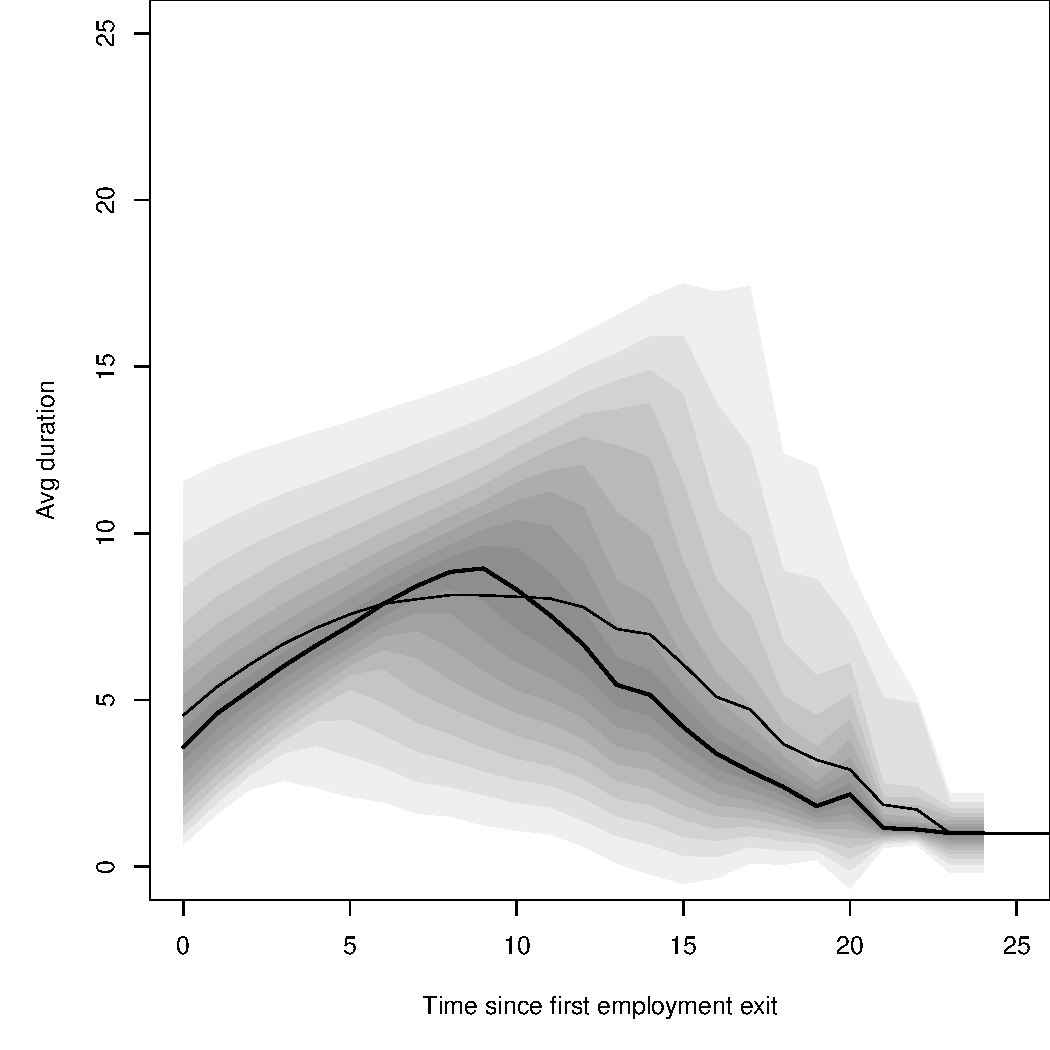
\includegraphics[scale=.4]{Figures/Macro2.pdf}
\end{subfigure}

\begin{subfigure}{.49\textwidth}
\centering
\caption{Time remaining in spell, mean vs quantiles.}
\label{fig:macro3}
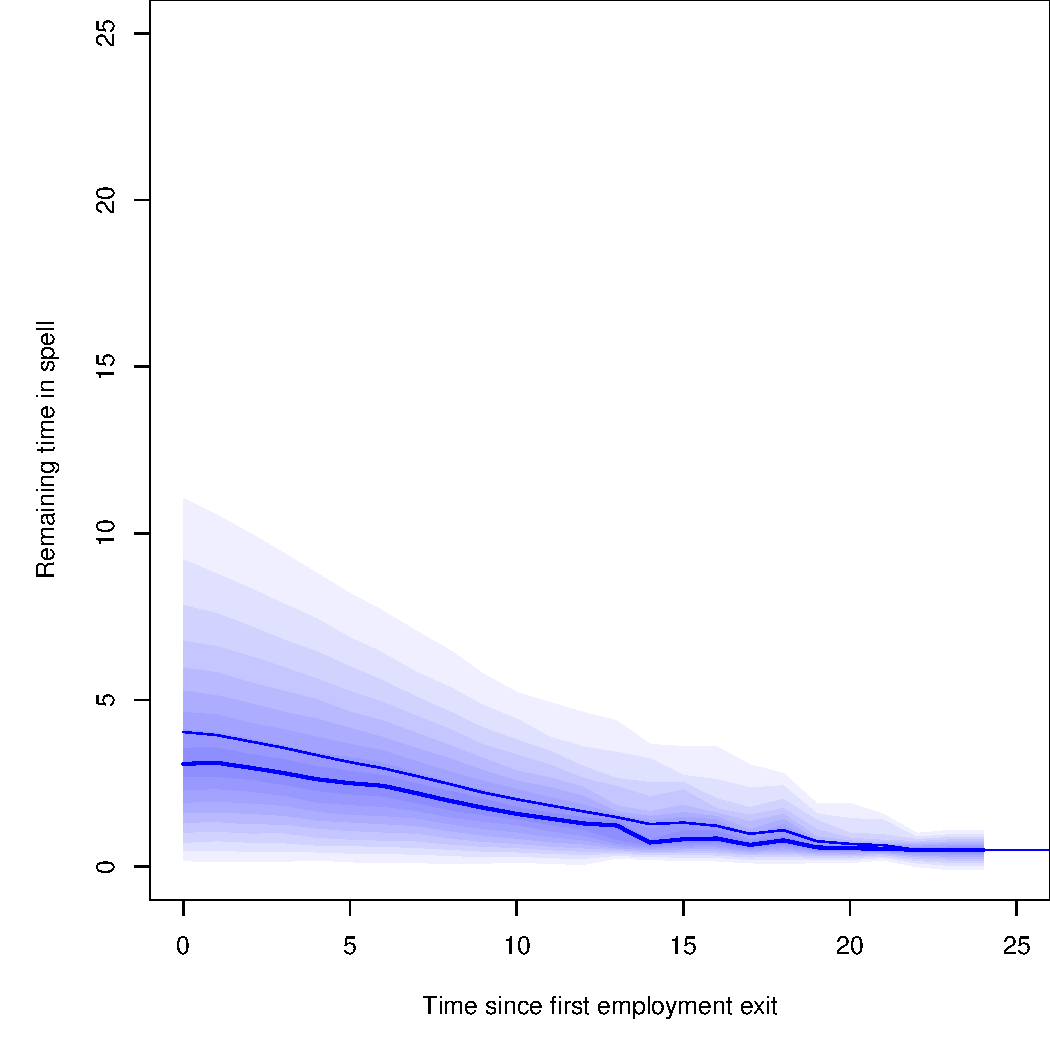
\includegraphics[scale=.4]{Figures/Macro3.pdf}
\end{subfigure}
~
\begin{subfigure}{.49\textwidth}
\centering
\caption{Time spent in spell, mean vs quantiles.}
\label{fig:macro4}
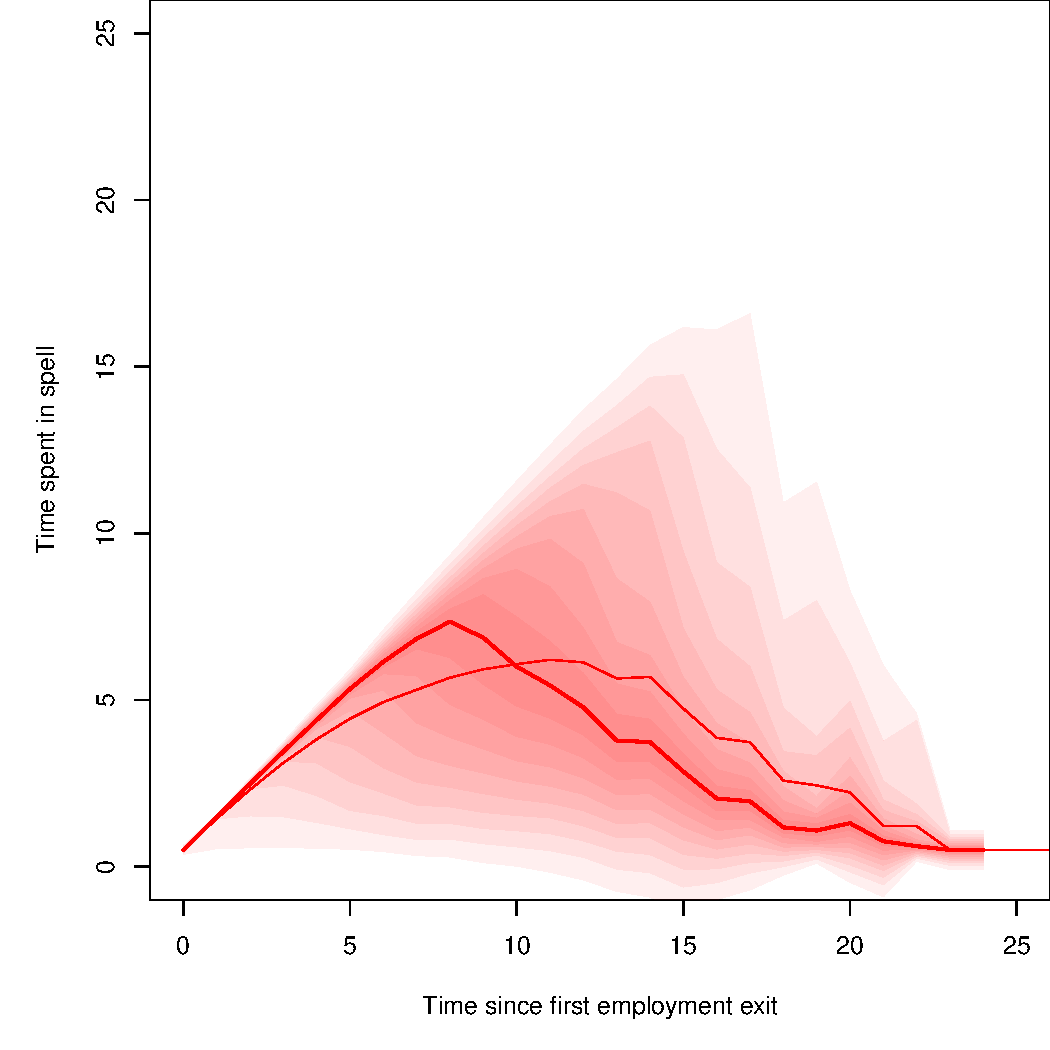
\includegraphics[scale=.4]{Figures/Macro4.pdf}
\end{subfigure}
\end{figure}


\section{Discussion}
Observe that the episode statistics displayed in Figure~\ref{fig:macrofirst},
inactivity spells structured by time since exit from one's first employment
spell, was chosen haphazardly. Let's say we have a process with 3 state
categories. Given one of these states, one may select the first, last, longest
or some other episode for purposes of alignment. For simplicity let's say we
have 3 choices like this for episode order. Alignment may then be left, right,
center, or something else, so let's say again for simplicity that there are 3
ways to align. Now we have 3 or 5 or more clock variables than might be worth
calculating statistics on structured like this. It should be clear that the
researcher easily has 100+ potential macro age-like patterns that might be
calculated, just for this relatively simple example case. It may be surprising
to behold that most of these patterns, even though they result from a simple markov
process with a small set of simple and monotonic age patterns, have some
character to them. They contain information. Presumably the age patterns that
entered into said markov model do not capture the entire story, and raw
observed state sequences are expected to bear stronger degrees of
codependency. And if we wish to know something about
episodes of the states we are studying, the researcher has i) large degrees of freedom in selecting macro episode patterns, and ii) is limited only by one's own creativity in doing so.

The researcher is not obliged to move in
the direction I propose, but the straw-man default scenario is to treat
episode structure (and any process for that matter) as if the only thing that matters is the
amount of time passed since birth. Where health, employment, or other life
events are co-dependent, the importance of age as a structural predictor is
expected to wane with respect to other transitions. Fetuses, babies, and
toddlers are largely synchronized with each other as a function of time until or
since birth. This is less so for children, whose development slowly begins to
lose alignment, far less so for young adults, some of which have passed through
first life transitions and others that have passed through none. Adults in mid
life and old age are maximally heterogenous with respect to age structure. To
gain further insight, it makes sense to realign.

As stated, the purpose of episode clocks and sequence realignment is to detect
important patterns in data (or model results) that are likely to otherwise
go unnoticed. Some reasonable priors might include that i) life course events
condition each other; ii) temporal proximity to life course transitions is likely to be an important
predictor of other transitions; iii) within-episode patterns of other
characteristics might be monotonically increasing or decreasing, or concave or
convex. Therefore, it may be the case that aggregate patterns derived from such
operations are simply sharper and of more obvious interpretation and consequence
than are age patterns themselves. 

It is difficult to offer advice on the judicious application of data
operations proposed here. All I can say is that the researcher should sit back
and think creatively about the process under study and not be afraid to
experiment some with clocks and alignment. The initial motivating case here
involved no re-alignment whatsoever: I just wanted to know how episode duration
changes over age. This very question already begs a second round of questions,
for it is unclear how to relate episodes to age, given that an age is a point
and an episode is a duration. This conundrum is what gives rise to clocks as an
operation. From there alignment is a natural next question, and the magnitude of
our researcher degrees of freedom increases by another order. In combination,
these steps already imply some distancing from markov matrix models, as even
cutting edge developments in this methodology are far from reaching the degree
of flexibility we propose to have.

\FloatBarrier
\singlespacing
\bibliographystyle{plainnat}
  \bibliography{references} 
\end{document}
